\documentclass[12pt, a4paper, twoside]{scrartcl}
 %---- Allgemeine Layout Einstellungen ------------------------------------------

% Für Kopf und Fußzeilen, siehe auch KOMA-Skript Doku
\usepackage[komastyle]{scrpage2}
\pagestyle{scrheadings}
\setheadsepline{0.5pt}[\color{black}]


%Einstellungen für Figuren- und Tabellenbeschriftungen
\setkomafont{captionlabel}{\sffamily\bfseries}
\setcapindent{0em}


%---- Weitere Pakete -----------------------------------------------------------
% Die Pakete sind alle in der TeX Live Distribution enthalten. Wichtige Adressen
% www.ctan.org, www.dante.de

% Sprachunterstützung
\usepackage[ngerman]{babel}

% Benutzung von Umlauten direkt im Text
% entweder "latin1" oder "utf8"
\usepackage[utf8]{inputenc}

% Pakete mit Mathesymbolen und zur Beseitigung von Schwächen der Mathe-Umgebung
\usepackage{latexsym,exscale,stmaryrd,amssymb,amsmath}

% Weitere Symbole
\usepackage[nointegrals]{wasysym}
\usepackage{eurosym}

% Anderes Literaturverzeichnisformat
%\usepackage[square,sort&compress]{natbib}

% Für Farbe
\usepackage{color}

% Zur Graphikausgabe
%Beipiel: \includegraphics[width=\textwidth]{grafik.png}
\usepackage{graphicx}

% Text umfließt Graphiken und Tabellen
% Beispiel:
% \begin{wrapfigure}[Zeilenanzahl]{"l" oder "r"}{breite}
%   \centering
%   \includegraphics[width=...]{grafik}
%   \caption{Beschriftung} 
%   \label{fig:grafik}
% \end{wrapfigure}
\usepackage{wrapfig}

% Mehrere Abbildungen nebeneinander
% Beispiel:
% \begin{figure}[htb]
%   \centering
%   \subfigure[Beschriftung 1\label{fig:label1}]
%   {\includegraphics[width=0.49\textwidth]{grafik1}}
%   \hfill
%   \subfigure[Beschriftung 2\label{fig:label2}]
%   {\includegraphics[width=0.49\textwidth]{grafik2}}
%   \caption{Beschriftung allgemein}
%   \label{fig:label-gesamt}
% \end{figure}
\usepackage{subfigure}

% Caption neben Abbildung
% Beispiel:
% \sidecaptionvpos{figure}{"c" oder "t" oder "b"}
% \begin{SCfigure}[rel. Breite (normalerweise = 1)][hbt]
%   \centering
%   \includegraphics[width=0.5\textwidth]{grafik.png}
%   \caption{Beschreibung}
%   \label{fig:}
% \end{SCfigure}
\usepackage{sidecap}
\usepackage{float}

% Befehl für "Entspricht"-Zeichen
\newcommand{\corresponds}{\ensuremath{\mathrel{\widehat{=}}}}
\newcommand{\folgt}{\ensuremath{\mathrel{\Rightarrow}}}
\newcommand{\equals}{\ensuremath{\mathrel{\Leftrightarrow}}}
\newcommand{\degree}{\ensuremath{\mathrel{^{\circ}}}}

\newcommand{\nn}{\nonumber}
\newcommand{\tn}[1]{\textnormal{#1}}
\newcommand{\D}{\ensuremath{\mathrel{\rm d}}}

\newcommand{\const}{\tn{const}}

\newcommand{\meter}{\ensuremath{\mathrel{\tn m}}}
\newcommand{\kilogramm}{\ensuremath{\mathrel{\tn{kg}}}}
\newcommand{\second}{\ensuremath{\mathrel{\tn s}}}
\newcommand{\sekunde}{\second}

\newcommand{\volt}{\ensuremath{\mathrel{\tn V}}}
\newcommand{\pascal}{\ensuremath{\mathrel{\tn{Pa}}}}
\newcommand{\coulomb}{\ensuremath{\mathrel{\tn C}}}
\newcommand{\newton}{\ensuremath{\mathrel{\tn N}}}
\newcommand{\liter}{\ensuremath{\mathrel{\tn l}}}
\newcommand{\celsius}{\ensuremath{\mathrel{\tn C}}}
\newcommand{\fahrenheit}{\ensuremath{\mathrel{\tn F}}}
\newcommand{\joule}{\ensuremath{\mathrel{\tn J}}}
\newcommand{\kelvin}{\ensuremath{\mathrel{\tn K}}}
\newcommand{\mol}{\ensuremath{\mathrel{\tn{mol}}}}
\newcommand{\gramm}{\ensuremath{\mathrel{\tn{g}}}}

\newcommand{\kilo}{\ensuremath{\mathrel{\tn k}}}
\newcommand{\hecto}{\ensuremath{\mathrel{\tn h}}}

\newcommand{\centi}{\ensuremath{\mathrel{ \tn c}}}
\newcommand{\milli}{\ensuremath{\mathrel{ \tn m}}}
\newcommand{\micro}{\ensuremath{\mathrel{ \tn\mu }}}



%\newcommand{}{\ensuremath{\mathrel{  }}}
%\newcommand{}{\ensuremath{\mathrel{  }}}
%\newcommand{}{\ensuremath{\mathrel{  }}}


\newcommand{\person}[1]{\textsc{#1}}

 \begin{document}
 %Titelseite
\begin{titlepage}
\centering
\textsc{\Large Anfängerpraktikum der Fakultät für
  Physik,\\[1.5ex] Universität Göttingen}

\vspace*{4.2cm}

\rule{\textwidth}{1pt}\\[0.5cm]
{\huge \bfseries
  Spezifische Wärme der Luft und Gasthermometer}\\[0.5cm]
\rule{\textwidth}{1pt}

\vspace*{3.5cm}

\begin{Large}
\begin{tabular}{ll}
Praktikanten: &  Silke Andrea Teepe\\
& Marcel Kramer\\
E-Mail: & \\
Betreuer: & Alexander Schmelev\\
\end{tabular}
\end{Large}

\vspace*{0.8cm}

\begin{Large}
\fbox{
  \begin{minipage}[t][2.5cm][t]{6cm} 
    Testat:
  \end{minipage}
}
\end{Large}

\end{titlepage}
\cleardoublepage
\tableofcontents
\cleardoublepage
\setcounter{page}{1}

\section{Einleitung}
\label{sec:einleitung}


\section{Theorie}
\label{sec:theorie}


\section{Durchführung}
\label{sec:durchfuehrung}
\subsection{Gasthermometer}
\begin{figure}
	\centering
	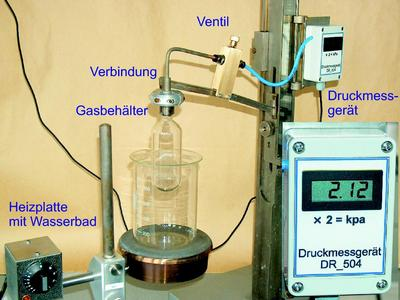
\includegraphics[scale=1]{Gasthermometer.png}
	\caption{Versuchsaufbau Gasthermometer \footnote{https://lp.uni-goettingen.de/get/text/3643 Abb.3723}}
\end{figure}
Da das Druckmessgerät nicht in der Lage ist, negative  Druckdifferenzen zu erfassen, wird zunächst das Ventil geöffnet und im Glaskolben Luftdruck hergestellt. Mit Hilfe von Eiswasser wird dann der Kolben auf etwa 0°C abgekühlt und anschließend das Ventil wieder verschlossen. Das Druckmessgerät sollte nun ca. 0,00kPa anzeigen. \\
Nun bestimmt man den Druck $p_V \left( T \right)$ der Luft im Kolben für konstantes Volumen $V$ und Temperaturen zwischen 0°C und 100°C, sowohl für Erwärmen, als auch Abkühlen des Kolbens. Dabei sollten Schritte von $\Delta T \le 5K $ gewählt werden. Um eine möglichste gleichförmige Temperaturänderung zu gewährleisten sollte das Wasserbad dauernd umgerührt werden.

\subsection{Spezifische Wärme der Luft}
\begin{figure}
	\centering
	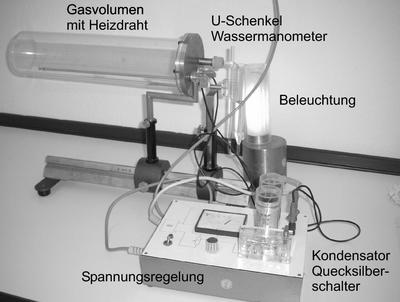
\includegraphics[scale=1]{SpezWaerme.png}
	\caption{Versuchsaufbau Spez. Wärme d. Luft \footnote{https://lp.uni-goettingen.de/get/text/3643 Abb.3724}}
\end{figure}
Ein Zylinder gefüllt mit Luft ist mit einem Wassermanometer verbunden. An dass Gasvolumen kann über einen Kondensator und einen Glühdraht eine spezifische Wärmemenge $Q$ abgegeben werden. Das Gasvolumen kann bei Vernachlässigung der Manometeränderung als konstant angesehen werden und somit die Druckänderung am Manometer abgelesen werden. \\
Der Kondensator wird aufgeladen und dann über den Heizdraht entladen. Dabei wird der maximale Ausschlag $\Delta p$ des Manometers abgelesen. Dieser wird für mehrfach für möglichst viele Spannungen zwischen 100V und 500V gemessen. Außerdem ist das Innenvolumen $V$ des Zylinders zu messen. \\
Während der Messung ist mit dem Ventil die Belüftungsöffnung des Zylinders zu verschließen und zwischen den Messungen beim Temperaturausgleich zu öffnen. Nach Beendigung der Messungen ist das Ventil geöffnet zurückzulassen.

\section{Auswertung}
\label{sec:auswertung}


\begin{table}
\centering
\begin{tabular}{r|c}
    Konstante & Wert\\
    $V_{Kolben}$ &  \\
    
 \end{tabular} 
 \caption{\label{tab:}Konstanten}
\end{table}


\begin{table}
\centering
\begin{tabular}{r|c|c|c|c|c|c|c|c|c|c|c|c|c|c|c|c|c|c|c|c}
    Temperatur$[\degree\celsius]$ & $0$ & $5$ & $10$ & $15$ &$20$ &$25$ &$30$ &$35$ &$40$ &$45$ &$50$ &$55$ &$60$ &$65$ &$70$ &$75$ &$80$ &$85$ &$90$ & $95$ & $100$\\
    Druck $[\kilo\pascal]$ &  $-0.07$ & $0.62$ & $ 1.41$ & $2.08$ & $2.75$ & $3.40$ & $4.01$ & $4.65$ & $5.28$ & $5.99$ & $6.62$ & $7.42$ & $8.16$ & $8.89$ & $9.56$ & $10.27$ & $10.95$ & $11.81$ & $12.15$ & $13.48$  \\
    
 \end{tabular} 
 \caption{\label{tab:}Erwärmen}
\end{table}

\begin{table}
\centering
\begin{tabular}{r|c|c|c|c|c|c|c|c|c|c|c|c|c|c|c|c|c|c|c|c}
    Temperatur$[\degree\celsius]$ & $100$ & $95$ & $90$ & $85$ & $80$ & $75$ & $70$ & $65$ & $60$ & $55$ & $50$ & $45$ & $40$ & $35$ & $30$ & $25$ & $20$ & $15$ & $10$ & $5$ & $0$ \\
    Druck $[\kilo\pascal]$ &  \\
    
 \end{tabular} 
 \caption{\label{tab:}Abkühlen}
\end{table}


%\begin{wraptable}{r}{5cm}
%\centering
%\begin{tabular}{r|l}
% \end{tabular} 
% \caption{\label{tab:}}
%\end{wraptable}

%\begin{table}
%\centering
%\begin{tabular}{r|c}
%    
% \end{tabular} 
% \caption{\label{tab:}}
%\end{table}


\section{Diskussion}
\label{sec:diskussion}

\end{document}
